\chapter [Introduction to Scilab]{Introduction to Scilab}


\section{AIM}
\begin{itemize}
\item
Study of SCILAB basics and getting familiar with the environment.
\item
Generation of various waveforms in continuous and discrete form.
\begin{itemize}
\item
Unit impulse signal
\item
Unit step signal
\item
Unit ramp signal
\item
Triangular signal
\item

Exponential signal
\item
Sinusoidal signal
\end{itemize}
\end{itemize}

\section{THEORY}
\paragraph{}

Scilab is an open source software for numerical mathematics and scientific visualization. It is capable of interactive calculations as well as automation of computations through programming. It provides all basic operations on matrices through built-in functions so that the trouble of developing and testing code for basic operations are completely avoided. Its ability to plot 2D and 3D graphs helps in visualizing the data we work with. All these make Scilab an excellent tool for teaching, especially those subjects that involve matrix operations. Further, the numerous toolboxes that are available for various specialized applications make it an important tool for research. Being compatible with Matlab®, all available Matlab M-files can be directly used in Scilab with the help of the Matlab to Scilab translator.Scicos, a hybrid dynamic systems modeler and simulator for Scilab, simplifies simulations. The greatest features of Scilab are that it is multiplatform and is free. It is available for many operating systems including Windows, Linux and MacOS X. \cite{scilab}
\paragraph{}

Scilab is a scientific software package which was developed since 1990 by researchers from INRIA(French National Institute for Research in Computer Science and Control) andENPC (National School of Bridges and Roads), it is now maintained anddeveloped by ScilabConsortium since its creation in May 2003 and integrated into Digiteo Foundation in July 2008. The current version is 5.5.1 (February2010).Since 1994 it is distributed freely along with source code through the Internet and is currently being used in educational and industrial environments around the world. From version 5 it is released under the GPL compatible CeCILL license.
\paragraph{}

When you start up Scilab, you see a window called Scilab console. The user enters Scilab commands at the prompt (-->). But many of thecommands are also availablethrough the menu at the top. Themost important menu for abeginner is the “Help” menu.Clicking on the “Help” menu opensup the Help Browser, showing alist of topics on which help isavailable. Clicking on the relevanttopic takes you to hyperlinkeddocuments similar to web pages. The codes for the programs are written as SciNotes by selecting a blank note from the tope top left corner of the Scilab Console.

\section{PROCEDURE}

\paragraph{}
\begin{enumerate}
\item
Start Scilab on PC and Scilab console window opens. Create a new blank SciNote.
\item
The code for the required program is typed and saved as Scilab SCE file with an extension .sci
\item

The continuous plots are made using the function “plot” and discrete plots are made using the function “plot2d3” with the corresponding x axis and y axis variables written inside().

\item
To view all the plots in the same window the function “subplot” is used.
\item
The results and the errors in the program are displayed in the console window.
The typed program is run using the “execute”.
\end{enumerate}

\section{SCILAB CODE}
\subsection*{Operations on discrete signals}


\lstinputlisting[title=Discrete Signals]{./scilabCode/discretesignals.sci}

\subsection*{Operations on continuous signals}
\lstinputlisting[title=Continuous Signals]{./scilabCode/continuoussignals.sci}

\section{RESULT}

\begin{enumerate}
\item
Familiarized SCILAB
\item
Basic experiments to generate different waveforms in discrete and continuous time domain were done. See Fig. \ref{discrete} and Fig. \ref{continuous}.
\end{enumerate}

The plotted figures are shown here.

\begin{figure}
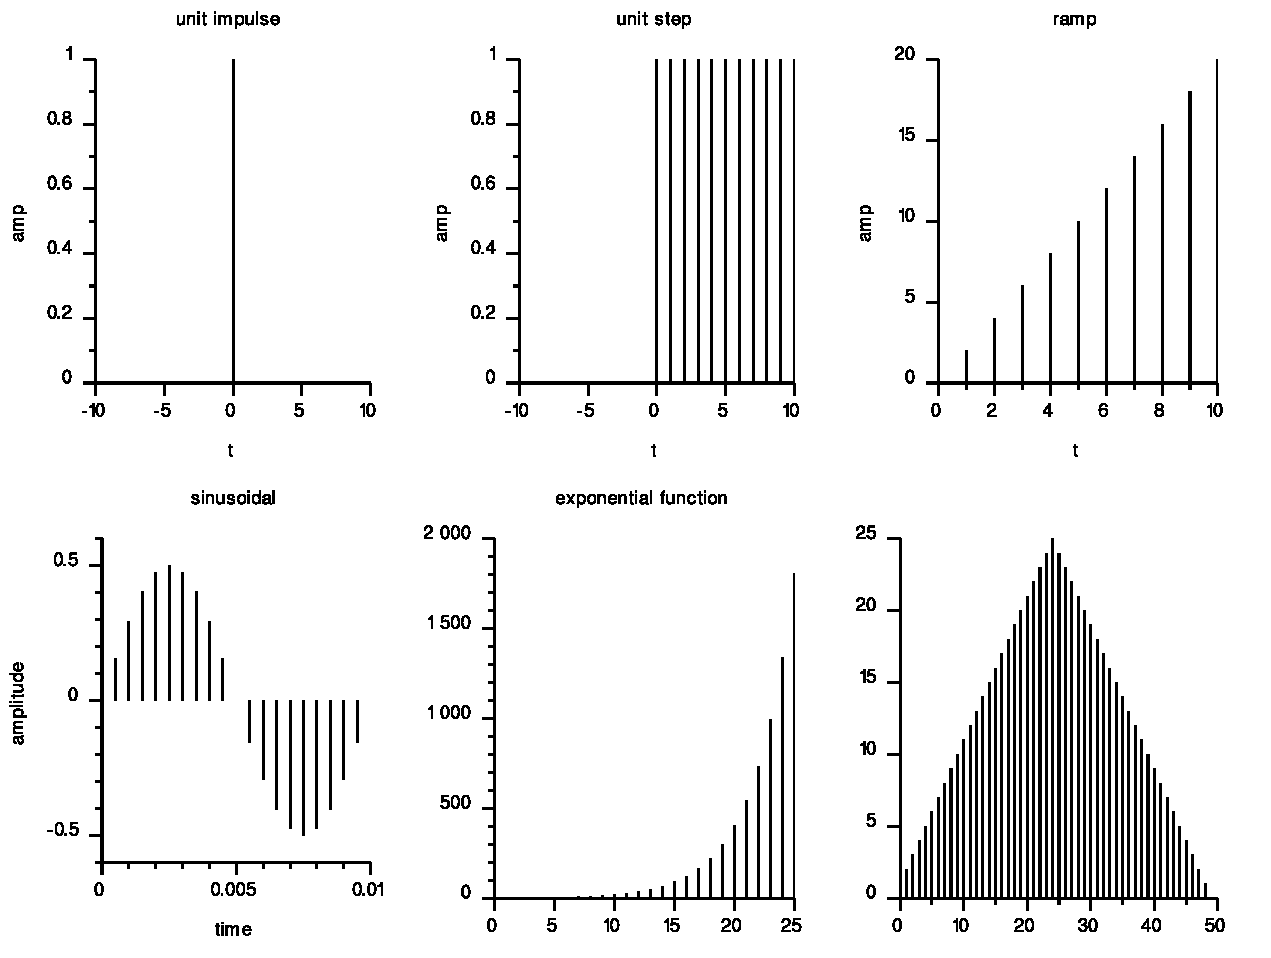
\includegraphics[scale=.5]{/home/kavya/kavyadev/DSPlab/scilabCode/discrete.pdf}

\caption{Plot of discrete signals}
\label{discrete}
\end{figure}

\begin{figure}
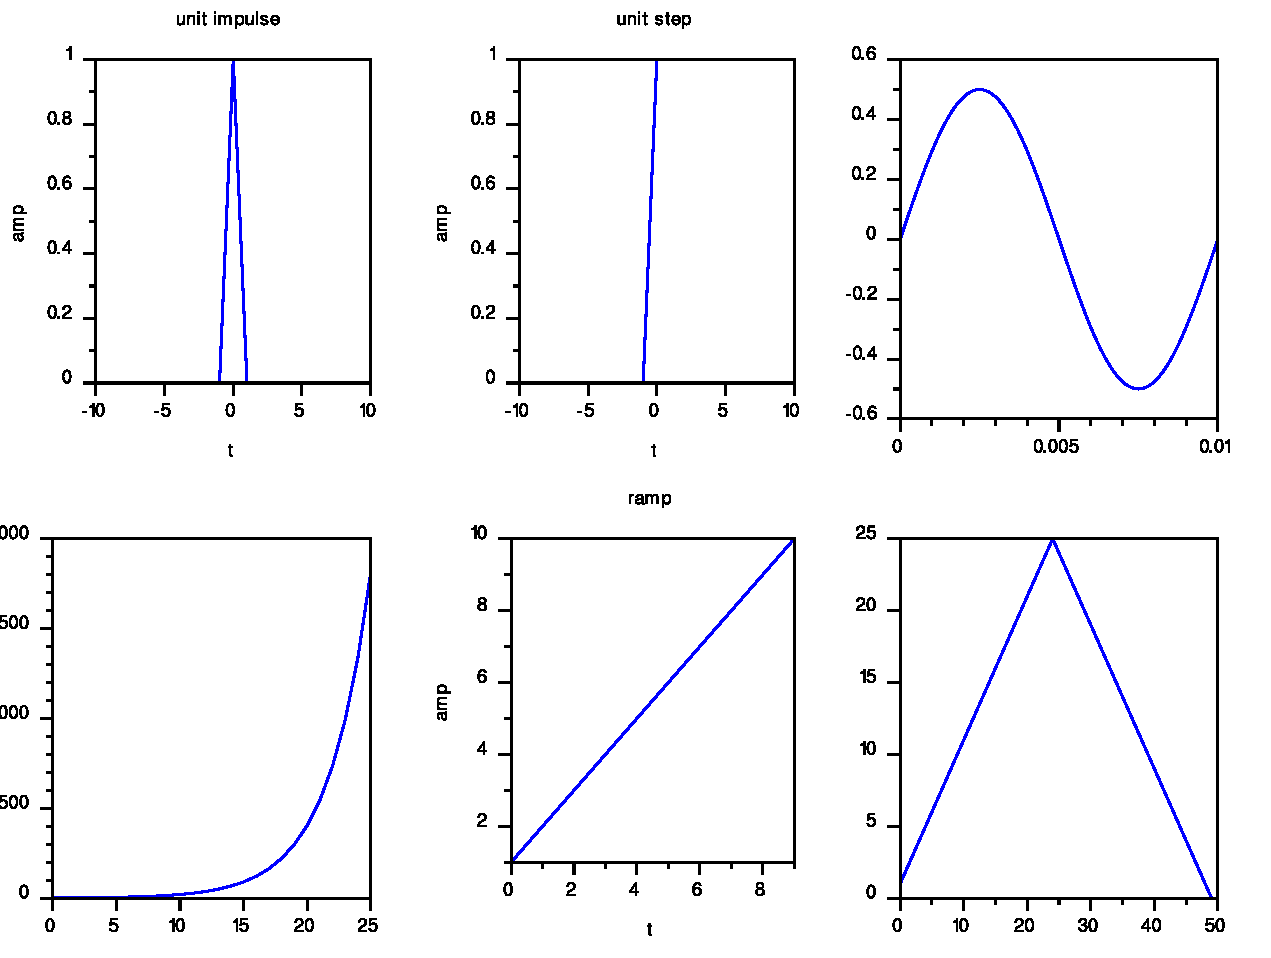
\includegraphics[scale=.5]{/home/kavya/kavyadev/DSPlab/scilabCode/continuous.pdf}
\caption{Plot of continuous signals}
\label{continuous}
\end{figure}
